% This file was created with tikzplotlib v0.10.1.
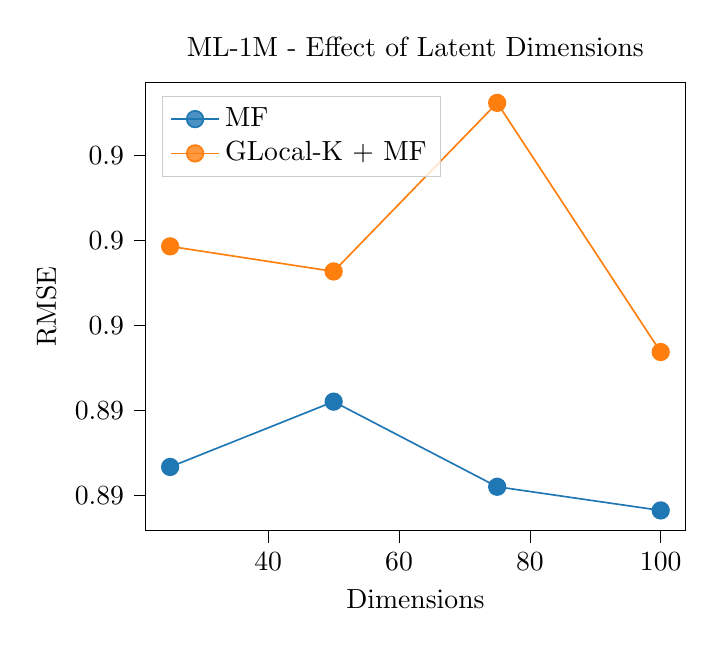
\begin{tikzpicture}

\definecolor{darkgray176}{RGB}{176,176,176}
\definecolor{darkorange25512714}{RGB}{255,127,14}
\definecolor{lightgray204}{RGB}{204,204,204}
\definecolor{steelblue31119180}{RGB}{31,119,180}

\begin{axis}[
legend cell align={left},
legend style={
  fill opacity=0.8,
  draw opacity=1,
  text opacity=1,
  at={(0.03,0.97)},
  anchor=north west,
  draw=lightgray204
},
tick align=outside,
tick pos=left,
title={ML-1M - Effect of Latent Dimensions},
x grid style={darkgray176},
xlabel={Dimensions},
xmin=21.25, xmax=103.75,
xtick style={color=black},
y grid style={darkgray176},
ylabel={RMSE},
ymin=0.8911680614, ymax=0.9017161066,
ytick style={color=black}
]
\addplot [semithick, steelblue31119180, mark=*, mark size=3, mark options={solid}]
table {%
25 0.892670214
50 0.894207239
75 0.892204463
100 0.891647518
};
\addlegendentry{MF}
\addplot [semithick, darkorange25512714, mark=*, mark size=3, mark options={solid}]
table {%
25 0.8978607
50 0.8972703
75 0.90123665
100 0.89537466
};
\addlegendentry{GLocal-K + MF}
\end{axis}

\end{tikzpicture}
